\subsection{Pantalla: Gestionar Áreas}
\subsubsection{Objetivo}
	El mapa de navegación se muestra en la Figura~\ref{fig:mapaNavegacionCU7}

   \begin{figure}[hbpt!]
 		\centering
 			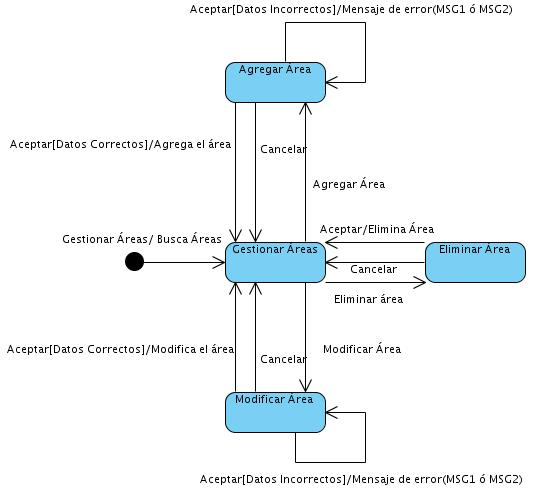
\includegraphics[width=0.8\textwidth]{images/CU7/MapaNavegacion.jpg}
 		\caption{Mapa de navegacion para el CU 7 Gestion de Areas.}
		\label{fig:mapaNavegacionCU7}
 	\end{figure}

\subsubsection{Objetivo}
Saber cuales son las áreas que están dadas de alta e interactuar con ellas. Vease Figura ~\ref{IUGestAreas} viene de Gestionar Catálogos.

\IUfig[0.6]{CU7/GestionArea.PNG}{IUGestAreas}{Gestionar Áreas.}

\subsubsection{Salidas}
Lista de Áreas Registradas.

\subsubsection{Controles}
\begin{itemize}
 \item \IUbutton{Flecha derecha} Muestra los siguientes n ejes temáticos.
 \item \IUbutton{Flecha izquierda} Muestra los n ejes temáticos anteriores.
\end{itemize}
\newpage
\subsubsection{Comandos}
\begin{itemize}
 \item \IUbutton{
\includegraphics[scale=0.2]{images/icons/agregar.png}} Muestra la ventana \IUref{IUAgregarArea}{Agregar Área}.
 \item \IUbutton{
\includegraphics[scale=0.15]{images/icons/eliminar.png}}:Lleva a la pantalla \IUref{IUEliminarArea}{Eliminar Área}, en donde se podrá eliminar el área de la fila donde se encuentra el botón. 
 \item \IUbutton{
\includegraphics[scale=0.15]{images/icons/editar.png}}: Permite modificar el área que corresponde a la fila de este botón, lleva a la pantalla \IUref{IUModificarArea}{Modificar Área}.

\end{itemize}


